\section{Motivation}
\label{Background}

In this section we discuss the most closely related work to our
proposed technique.  The idea of prefetching begins with Jouppi's
\textit{Instruction Stream Buffers}~\cite{ISB}. Early prefetchers
detected stride access patterns in order to predict future memory
requests~\cite{Smith,Baer,Stride}. Modern prefetching mechanisms are
more sophisticated as they look into past memory
behavior~\cite{Address_Correlated,AMPM},
locality~\cite{Spatial_Pattern,SMS,Temporal_Instruction_Fetch,Off_Chip,STMS,SMS_JILP},
control-flow speculation~\cite{BFetch,MTBFetch}, and other other
aspects to detect complex memory access patterns.  See
Section~\ref{related} for other relevant work.

\subsection{Underlying Prefetcher: SPP}
\label{Background-SPP}

Kim {\em et. al.} proposed Signature Path Prefetcher (SPP)~\cite{SPP},
a confidence-based lookahead prefetcher.  SPP creates a signature
associated with a page address by compressing the history of
accesses. By correlating the signature with future likely delta
patterns, SPP learns both simple and complicated memory access
patterns quickly.  While the basic idea of perceptron based prefetch
filtering is applicable to any lookahead prefetcher, we develop a
practical implementation of our proposed prefetch filter
using SPP as our underlying mechanism. 
Here we describe the basic architecture of SPP.
\newline
\newline
\noindent \textbf{Signature Table:} As shown on the left side of
Figure~\ref{fig:spp_update}, the Signature Table (ST) keeps track of 256
most recently accessed pages. It is meant to capture memory access
patterns within a page boundary. SPP indexes into an entry of the
Signature Table using the page number. For each entry corresponding to
a page, the table stores a `last block offset' and an `old
signature'. Last block offset is the block offset of the last memory
access of that given page. The block offset is calculated with respect
to the page boundary. The signature is a 12-bit compressed
representation of the past few memory accesses for that page. The
signature is calculated as:
$$New Signature = (\,Old Signature << 3 bits\,) \;\;XOR\;\;
(\,Delta\,)$$ Delta is the numerical difference between the block
offset of the current and the previous memory access. In case a
matching page entry is found, the stored signature retrieved and used
to index into the Pattern Table.  This process is illustrated in
Figure~\ref{fig:spp_update}.
\newline
\newline
\noindent \textbf{Pattern Table:} The Pattern Table (PT), shown on the right
side in Figure~\ref{fig:spp_update} is indexed by the signature
generated from the Signature Table.  Pattern Table holds predicted
delta patterns and their confidence estimates. Each entry indexed by
the signature holds up to 4 unique delta predictions.
%
\newline
\newline
\noindent \textbf{Lookahead Prefetching:} On each trigger, SPP goes
down the program speculation path using its own prefetch suggestion.
Using the current prefetch as a starting point, it re-accesses the Pattern
Table to generate further prefetches.  As illustrated in
Figure~\ref{fig:spp_structure}, it repeats the cycle of accessing
the PT and updating the signature based on highest confidence
prefetch from the last iteration.  The iteration counter on which SPP
manages to predict prefetch entries in the lookahead manner is
characterized as its `depth'. While doing so, SPP also keeps
compounding the confidence in each depth. Thus as depth increases,
overall confidence keeps decreasing.
\newline
\newline
\noindent \textbf{Confidence Tracking}: As shown in
Figure~\ref{fig:spp_structure}, the Pattern Table keeps a count of
hits to each signature through a counter C\textsubscript{sig}. The
number of hits for a given delta per signature are tracked using a
counter C\textsubscript{delta}.  The confidence for a given delta is
approximated through C\textsubscript{d} = C\textsubscript{delta} /
C\textsubscript{sig}.  When SPP enters into a lookahead mode, the path
confidence P\textsubscript{d} is:
$$P\textsubscript{d} \;=\; \alpha  \;.\;  C\textsubscript{d}  \;.\;
P\textsubscript{d-1}$$ Here $\alpha$ represents the global accuracy,
calculated as the ratio of the number of prefetches which led to a
demand hit to the number of prefetches recommended in total. The range
of $\alpha$ is [0,1].  The lookahead depth is represented by $d$. 
For $d = 1$, when
SPP is in non-speculative mode, P\textsubscript{0} can be thought of
as 1.  The final P\textsubscript{d} is thresholded against prefetch
threshold (T\textsubscript{p}) to reject the low confidence
suggestions and then against a numerically bigger fill threshold
(T\textsubscript{f}) to decide whether to send the prefetch to
L2 Cache (high confidence prefetch) or Last Level Cache (low
confidence prefetch). The two thresholds were empirically set to 25
and 90 respectively, on the scale of 0 to 100.

\begin{figure}
  \begin{center}
  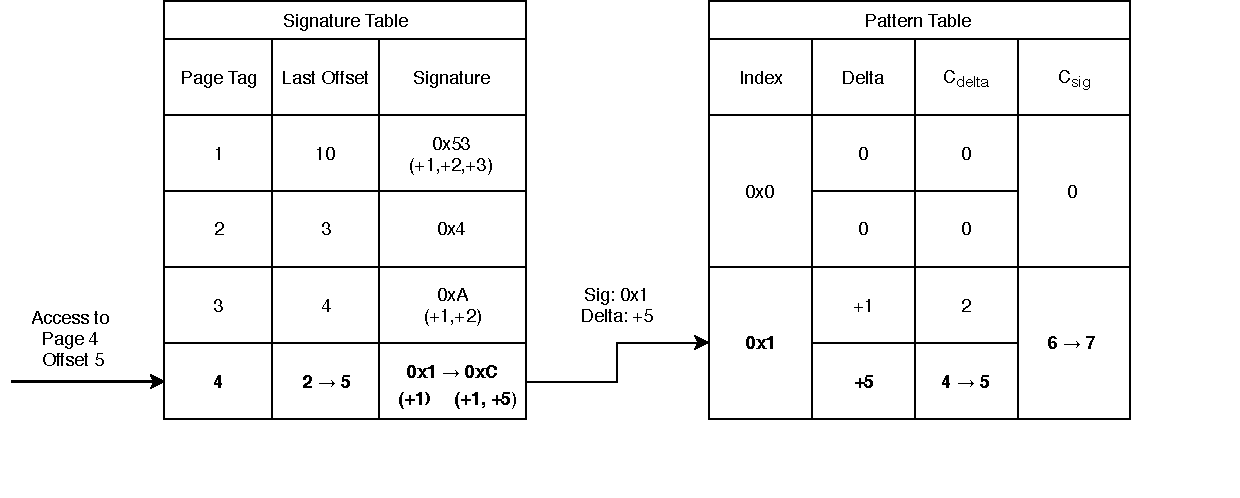
\includegraphics[width=\columnwidth]{SPP_Update_Description}
  \caption{SPP Data-path Flow}
  \label{fig:spp_update}
  \end{center}
\end{figure}


\begin{figure}
  \begin{center}
  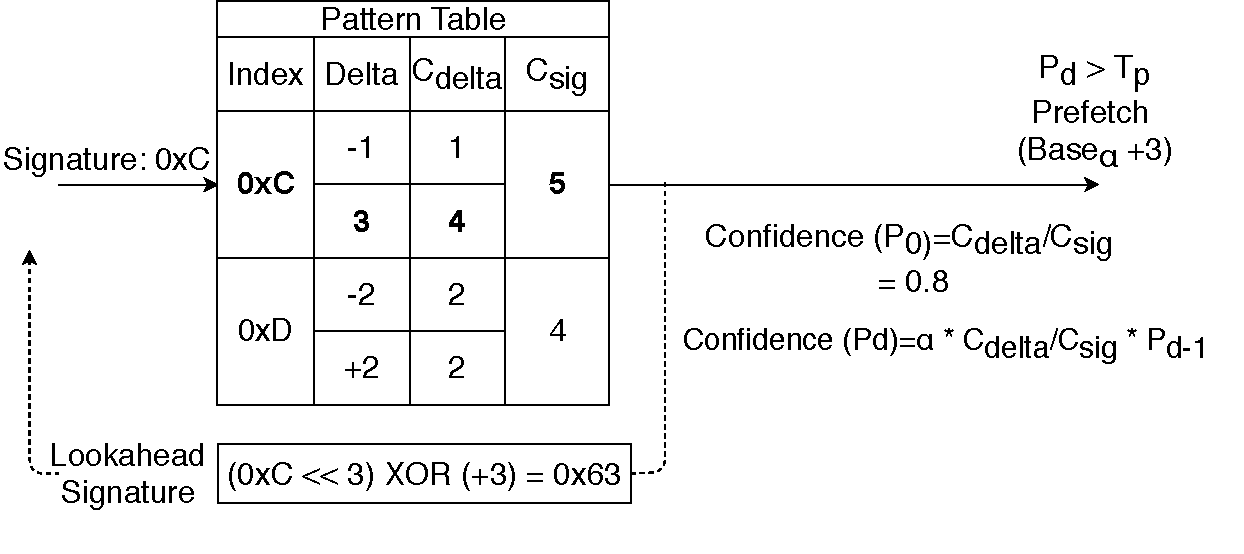
\includegraphics[width=\columnwidth]{SPP_Prefetch_Description}
  \caption{SPP Architecture}
  \label{fig:spp_structure}
  \end{center}
\end{figure}

\subsection{Case for an On-line Filter}
\label{Background-Case}

As was noted in Figure~\ref{Fig:Motivation}, aggressive lookahead
prefetching, if done without any accuracy check, can harm the
performance of the system. As the figure shows, aggressive lookahead
and its accompanied loss of accuracy degrades performance by almost
9\%.  This is despite a growing number of useful prefetches generated
by the prefetcher.  Thus, we need a mechanism that is orthogonal to
the underlying prefetching scheme and can be used to prune out the
useful prefetches from the useless ones.

Moreover, the on-line confidence mechanism used by most prefetchers is
very rudimentary. For example, SPP's internal confidence mechanism is
based on taking the ratio C\textsubscript{d} = C\textsubscript{delta}
/ C\textsubscript{sig}. This confidence was used to make the decision
of whether to prefetch or not to prefetch; and which level to
prefetch.  While this approximation was shown to work in the original
implementation, we believe that a better form of generalized on-line
decision making is possible. Hence, it was necessary to build a
robust and adaptable learning mechanism to accept / reject the
prefetch suggestions, and to decide the fill level (L2 Cache vs Last
Level Cache). Thus, we introduce an independent on-line perceptron
based filtering mechanism.

\subsection{Perceptron Learning}
\label{sec:Background-Perceptron}
Perceptron learning for microarchitectural prediction was introduced
for branch prediction~\cite{PerceptronPredictor}. Our predictor uses a
version of microarchitectural perceptron prediction known as the
``hashed perceptron'' organization~\cite{HashedPerceptron}. As an
abstract idea, a hashed perceptron predictor hashes several different
features into values that index several distinct tables. Small integer
weights are read out from the tables and summed. If the sum exceeds
some threshold, a positive prediction is made, {\em e.g.} ``predict
branch taken'' or ``allow the prefetch.'' Otherwise, a negative
prediction is made. Once the ground truth is known, the weights
corresponding to the prediction are incremented if the outcome was
positive, or decremented if it was negative. This update only occurs
if the prediction was incorrect or if the magnitude of the sum failed
to exceed a threshold.  Beyond branch prediction, perceptron learning
has been applied to last-level cache reuse
prediction~\cite{Perc_Reuse,Multiperspective}. In this paper, we apply
it for the first time to do prefetch filtering.
